\section{Requerimientos funcionales}
Los requerimientos funcionales describen las actividades o los comportamientos que el sistema debe realizar cuando se cumplen ciertas condiciones.
\\
A continuación, se presenta un listado con los requerimientos funcionales que se obtuvieron del sistema.
El listado de requerimientos funcionales se encuentra dividido de acuerdo con los módulos que se identificaron.

\paragraph{}
\begin{figure}[H]
	\centering
	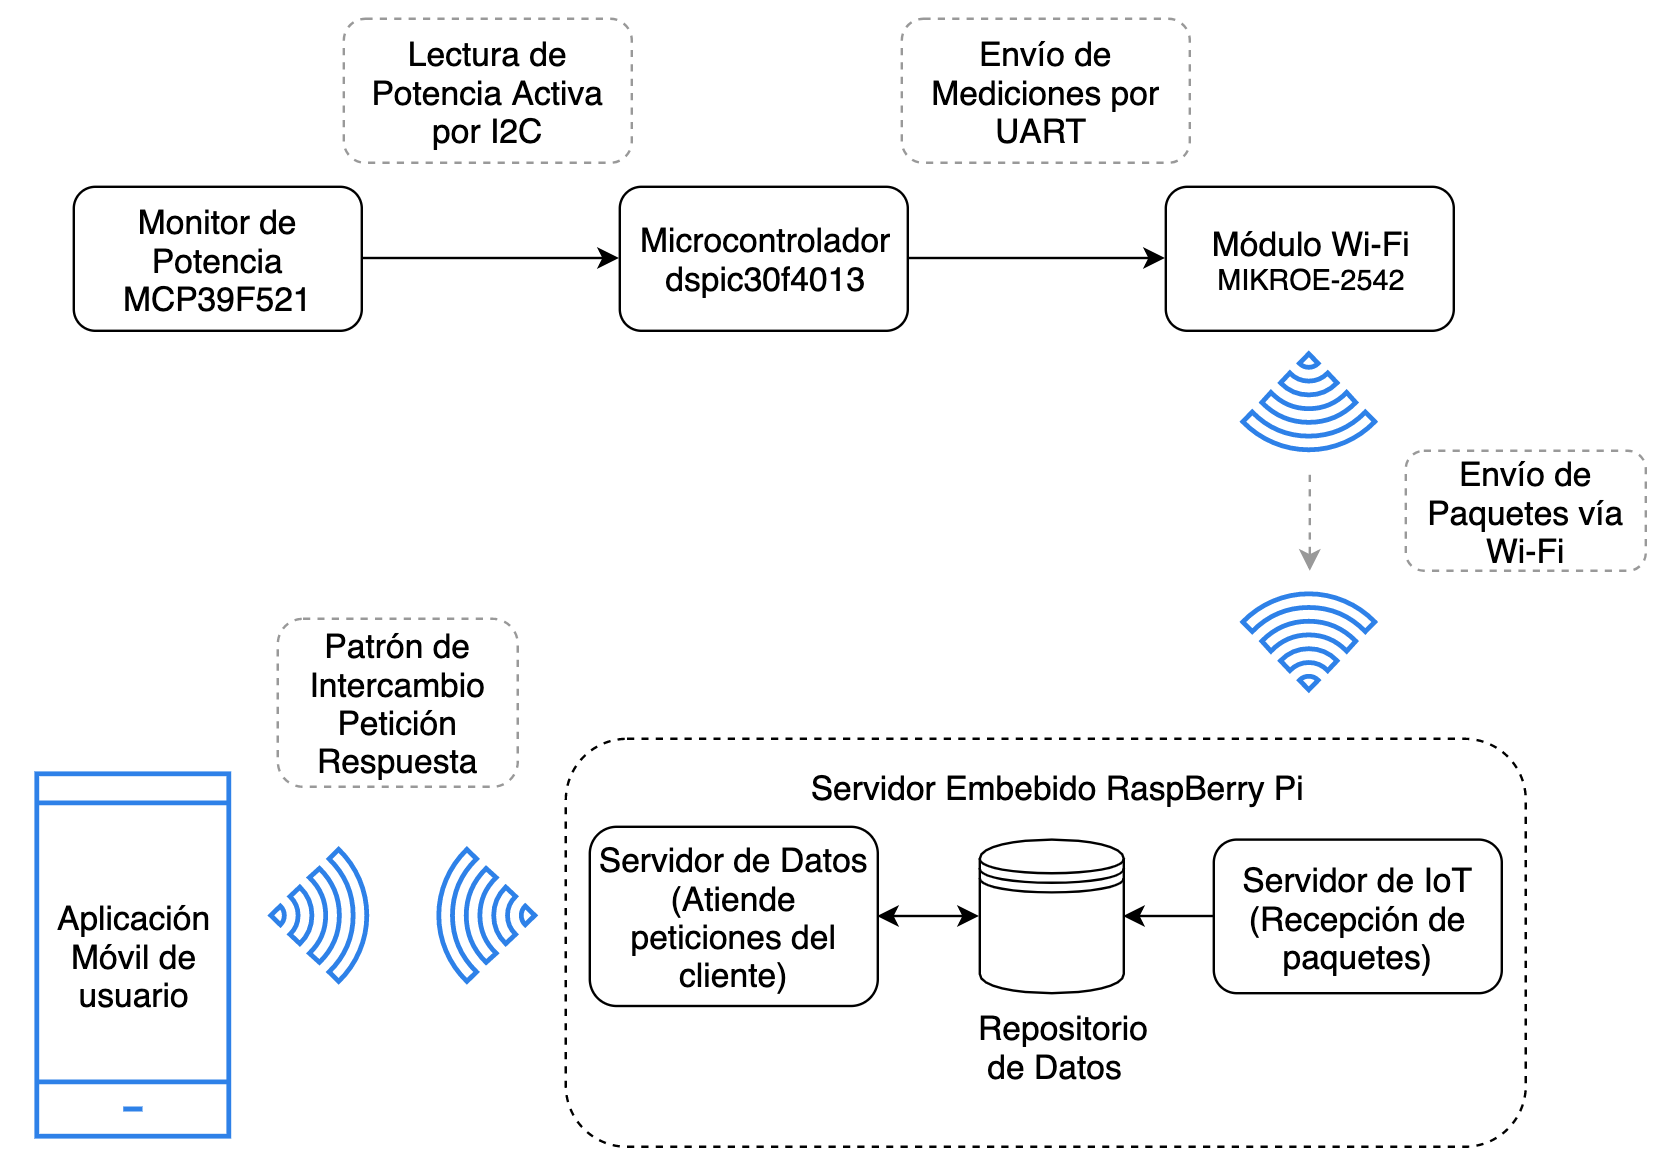
\includegraphics[scale=.4]{Capitulo3/img/diagramabloques.png}
	\caption{Diagrama a bloques del sistema}
	\label{fig:diagrama_dispMonitoreo}
\end{figure}

\begin{itemize}
	\item Módulo de Microcontrolador.
	\item Módulo de Servidor.
	\item Módulo de Aplicación de usuario.
\end{itemize}

\paragraph{Módulo de Microcontrolador}.
%\begin{enumerate}[label=RF\arabic*]
%	\item Proporcionar un mecanismo de comunicación vía IIC desde el sensor MCP39F521 hacia el microcontrolador DSPIC30F4013.
%	\item Proporcionar un mecanismo de comunicación vía UART desde el microcontrolador DSPIC30F4013 hacia el módulo Wi-Fi MIKROE-2542.
%\end{enumerate}
\begin{longtable}{|M{1.6cm}|M{4.0cm}|M{6.0cm}|}
    \caption{Requerimientos funcionales del módulo de microcontrolador}
	\hline
	\textbf{RF} & \textbf{Nombre} & \textbf{Descripción} \\ 
	\hline
 	\begin{enumerate}[label=RF\arabic*]
 	    \item.
 	\end{enumerate}
 	& Comunicación sensor-microcontrolador
 	& El sistema deberá contar con un mecanismo de comunicación vía IIC desde el microcontrolador DSPIC30F4013 hacia el sensor MCP39F521. \\
    \hline
    \begin{enumerate}[label=RF\arabic*]
        \setcounter{enumi}{1}
 	    \item.
 	\end{enumerate}
 	& Comunicación microcontrolador-módulo WiFi
 	& El sistema deberá contar con un mecanismo de comunicación vía UART desde el microcontrolador DSPIC30F4013 hacia el módulo Wi-Fi MIKROE-2542 para el envío de muestras en paquetes UDP. \\
    \hline
\end{longtable}



\paragraph{Módulo de Servidor}.
%\begin{enumerate}[label=RF\arabic*.]
%	\setcounter{enumi}{2}
%	\item Proporcionar un servicio para la recepción de los paquetes enviados por el módulo Wi-Fi MIKROE-2542 y su almacenamiento en un archivo de formato de texto.
%	\item Proporcionar un servicio de comunicación vía HTTP para el envío de la información almacenada para dar respuesta a las peticiones realizadas por el usuario desde la aplicación móvil.  
%\end{enumerate}
\begin{longtable}{|M{1.6cm}|M{4.0cm}|M{6.0cm}|}
    \caption{Requerimientos funcionales del módulo de servidor}
	\hline
	\textbf{RF} & \textbf{Nombre} & \textbf{Descripción} \\ 
	\hline
 	\begin{enumerate}[label=RF\arabic*]
 	    \setcounter{enumi}{2}
 	    \item.
 	\end{enumerate}
 	& Servicio para la recepción de paquetes del módulo Wi-Fi
 	& El sistema deberá proporcionar un servicio para la recepción de los paquetes UDP enviados por el módulo Wi-Fi MIKROE-2542 y su almacenamiento en un archivo de formato JSON.\\
    \hline
    \begin{enumerate}[label=RF\arabic*]
        \setcounter{enumi}{3}
 	    \item.
 	\end{enumerate}
 	& Servicio de comunicación vía TCP/IP
 	& El sistema deberá proporcionar un servicio de comunicación vía TCP/IP para el envío de la información almacenada en el servidor que será solicitada por medio de las peticiones realizadas por el usuario desde la aplicación móvil. \\
    \hline
\end{longtable}



\paragraph{Módulo de Aplicación de usuario}.
%\begin{enumerate}[label=RF\arabic*.]
%	\setcounter{enumi}{4}
%	\item Proporcionar un mecanismo para la vinculación entre la aplicación y el servidor.
%	\item Proporcionar un servicio de comunicación vía HTTP para la generación de peticiones al servidor.
%	\item Proporcionar un mecanismo para la visualización en tiempo real de la generación  de la energía producida por el sistema fotovoltaico.
%	\item Proporcionar un mecanismo para la generación de estadísticas de la producción de energía por el sistema fotovoltaico.
%	\item Informar por medio de notificaciones cuando el sistema fotovoltaico dejó de producir energía, así como al final del día notificar si se produjo más o menos energía que el promedio diario de producción.  
%\end{enumerate}
\begin{longtable}{|M{1.6cm}|M{4.0cm}|M{6.0cm}|}
    \caption{Requerimientos funcionales del módulo de aplicación de usuario}
	\hline
	\textbf{RF} & \textbf{Nombre} & \textbf{Descripción} \\
	\hline
 	\begin{enumerate}[label=RF\arabic*]
 	    \setcounter{enumi}{4}
 	    \item.
 	\end{enumerate}
 	& Vinculación de aplicación con servidor.
 	& El usuario será capaz de vincular la aplicación móvil con el servidor siempre y cuando proporcione un correo electrónico y una contraseña (en el caso de ser la primera vez que se vincula) o bien la contraseña establecida al inicio (para las próximas veces que se vincula).\\
    \hline
    \begin{enumerate}[label=RF\arabic*]
        \setcounter{enumi}{5}
 	    \item.
 	\end{enumerate}
 	& Comunicación servidor-aplicación de usuario 
 	& El sistema deberá proporcionar un servicio de comunicación vía TCP/IP para la generación de peticiones de la aplicación móvil hacia el servidor. \\
    \hline
    \begin{enumerate}[label=RF\arabic*]
        \setcounter{enumi}{6}
 	    \item.
 	\end{enumerate}
 	& Monitoreo en Tiempo real 
 	& El usuario será capaz de visualizar gráficas con información que se obtiene en tiempo real sobre la generación de energía del sistema fotovoltaico por cada uno de los nodos conectados al servidor. \\
    \hline
    \begin{enumerate}[label=RF\arabic*]
        \setcounter{enumi}{7}
 	    \item.
 	\end{enumerate}
 	& Monitoreo Histórico 
 	& El usuario será capaz de visualizar gráficas con información que se obtuvo en periodos de tiempo anteriores sobre la generación de energía del sistema fotovoltaico por cada uno de los nodos conectados al servidor. \\
    \hline
    \begin{enumerate}[label=RF\arabic*]
        \setcounter{enumi}{8}
 	    \item.
 	\end{enumerate}
 	& Estadísticas de la producción de energía 
 	& El sistema deberá ser capaz de recolectar, clasificar y hacer cálculos con la información obtenida de la producción de energía del sistema fotovoltaico. \\
    \hline
    \begin{enumerate}[label=RF\arabic*]
        \setcounter{enumi}{9}
 	    \item.
 	\end{enumerate}
 	& Notificaciones del Sistema fotovoltaico 
 	& Si el usuario habilita las notificaciones desde la aplicación móvil, el sistema deberá informar por medio de notificaciones cuando el sistema fotovoltaico dejó de producir energía, cuando no se está obteniendo información de un nodo o cuando no se recibe respuesta del servidor. \\
    \hline
    \begin{enumerate}[label=RF\arabic*]
        \setcounter{enumi}{10}
 	    \item.
 	\end{enumerate}
 	& Listado de servidores vinculados 
 	& El usuario podrá visualizar un listado de los servidores que ha vinculado por medio de la aplicación móvil y por cada servidor tiene las opciones de obtener su contraseña vía email, editar el nombre del servidor y eliminar el servidor del listado. \\
    \hline
    \begin{enumerate}[label=RF\arabic*]
        \setcounter{enumi}{11}
 	    \item.
 	\end{enumerate}
 	& Listado de notificaciones recibidas 
 	& El usuario podrá visualizar un listado de las últimas 100 notificaciones que ha recibido en el dispositivo móvil. \\
    \hline
    
\end{longtable}